% -----------------------------------------------
% Template for SMC 2020
% adapted from previous SMC paper templates
% -----------------------------------------------

\documentclass{article}
\usepackage{smc2020}
\usepackage{times}
\usepackage{ifpdf}
\usepackage[english]{babel}
\usepackage{cite}
\usepackage{amsmath}
\usepackage{tabularx}
\usepackage{listings}

%%%%%%%%%%%%%%%%%%%%%%%% Some useful packages %%%%%%%%%%%%%%%%%%%%%%%%%%%%%%%
%%%%%%%%%%%%%%%%%%%%%%%% See related documentation %%%%%%%%%%%%%%%%%%%%%%%%%%
%\usepackage{amsmath} % popular packages from Am. Math. Soc. Please use the 
%\usepackage{amssymb} % related math environments (split, subequation, cases,
%\usepackage{amsfonts}% multline, etc.)
%\usepackage{bm}      % Bold Math package, defines the command \bf{}
%\usepackage{paralist}% extended list environments
%%subfig.sty is the modern replacement for subfigure.sty. However, subfig.sty 
%%requires and automatically loads caption.sty which overrides class handling 
%%of captions. To prevent this problem, preload caption.sty with caption=false 
%\usepackage[caption=false]{caption}
%\usepackage[font=footnotesize]{subfig}


%user defined variables
\def\papertitle{Applied Physical Modeling for Sound Synthesis:\linebreak The Yaybahar}
\def\firstauthor{Pelle Juul Christensen}
\def\secondauthor{Second author}
\def\thirdauthor{Third author}

% adds the automatic
% Saves a lot of output space in PDF... after conversion with the distiller
% Delete if you cannot get PS fonts working on your system.

% pdf-tex settings: detect automatically if run by latex or pdflatex
\newif\ifpdf
\ifx\pdfoutput\relax
\else
   \ifcase\pdfoutput
      \pdffalse
   \else
      \pdftrue
\fi

\ifpdf % compiling with pdflatex
  \usepackage[pdftex,
    pdftitle={Applied Physical Modeling for Sound Synthesis: The Yaybahar},
    pdfauthor={\firstauthor, \secondauthor, \thirdauthor},
    bookmarksnumbered, % use section numbers with bookmarks
    pdfstartview=XYZ % start with zoom=100% instead of full screen; 
                     % especially useful if working with a big screen :-)
   ]{hyperref}
  %\pdfcompresslevel=9

  \usepackage[pdftex]{graphicx}
  % declare the path(s) where your graphic files are and their extensions so 
  %you won't have to specify these with every instance of \includegraphics
  \graphicspath{{./figures/}}
  \DeclareGraphicsExtensions{.pdf,.jpeg,.png}

  \usepackage[figure,table]{hypcap}

\else % compiling with latex
  \usepackage[dvips,
    bookmarksnumbered, % use section numbers with bookmarks
    pdfstartview=XYZ % start with zoom=100% instead of full screen
  ]{hyperref}  % hyperrefs are active in the pdf file after conversion

  \usepackage[dvips]{epsfig,graphicx}
  % declare the path(s) where your graphic files are and their extensions so 
  %you won't have to specify these with every instance of \includegraphics
  \graphicspath{{./figures/}}
  \DeclareGraphicsExtensions{.eps}

  \usepackage[figure,table]{hypcap}
\fi

%setup the hyperref package - make the links black without a surrounding frame
\hypersetup{
    colorlinks,%
    citecolor=black,%
    filecolor=black,%
    linkcolor=black,%
    urlcolor=black
}


% Title.
% ------
\title{\papertitle}

% Authors
% Please note that submissions are NOT anonymous, therefore 
% authors' names have to be VISIBLE in your manuscript. 
%
% Single address
% To use with only one author or several with the same address
% ---------------
\oneauthor
  {\firstauthor} {Sound and Music Computing, Aalborg University, Copenhagen \\ %
    {\tt \href{mailto:pjch17@student.aau.dk}{pjch17@student.aau.dk}}}

%Two addresses
%--------------
% \twoauthors
%   {\firstauthor} {Affiliation1 \\ %
%     {\tt \href{mailto:author1@smcnetwork.org}{author1@smcnetwork.org}}}
%   {\secondauthor} {Affiliation2 \\ %
%     {\tt \href{mailto:author2@smcnetwork.org}{author2@smcnetwork.org}}}

% Three addresses
% --------------
%  \threeauthors
%    {\firstauthor} {Affiliation1 \\ %
%      {\tt \href{mailto:author1@smcnetwork.org}{author1@smcnetwork.org}}}
%    {\secondauthor} {Affiliation2 \\ %
%      {\tt \href{mailto:author2@smcnetwork.org}{author2@smcnetwork.org}}}
%    {\thirdauthor} { Affiliation3 \\ %
%      {\tt \href{mailto:author3@smcnetwork.org}{author3@smcnetwork.org}}}


% ***************************************** the document starts here ***************
\begin{document}
%
\capstartfalse
\maketitle
\capstarttrue
%
\begin{abstract}
Much work has been done on the theoretical aspects of physical modeling for sound synthesis and lots of models exist that can be combined to form larger acoustical systems.
In this paper I use those results to model a specific instrument, the Yaybahar, invented by Turkish artist Görkem Şen.
Each part of the instrument is covered independently and their physics are explained in an intuitive manner.
I then show how each model can be solved numerically using the method of finite difference schemes, which are reviewed briefly.
The models are implemented in C++ to form an interactive, real-time application, whose architecture and optimization is also discussed.
\end{abstract}
%

\section{Introduction}\label{sec:introduction}
\nocite{Someone:00}

The Yaybahar is a novel acoustical instrument invented by Turkish artist Görkem Şen.
It consists of a string connected to two springs that in turn, respectively, connect to two drum heads.
The instrument is played by bowing the string and striking the springs and drums using a mallet.
The combination of the springs and the drums create a grand, echoey, and reverberant sound that is not found in any other instruments (to my knowledge).
A video of Görkem Şen can be viewed on YouTube\footnote{\url{https://youtu.be/_aY6TxC1ojA}}.

In this paper we are going to see how to build a real-time sound synthesis algorithm that mimics the Yaybahar by using \textit{physical modeling}.

Many methods for physical modeling exists, some of them, such as digital wave guides and modal synthesis, results in great, high quality sounds, but might lack the nuance of the real instrument.
The method we are going to use is \textit{finite difference schemes} (FDS), which enable us to implement a proper numerical simulation of our instrument.

Finite difference schemes is a very mature method that has its roots in physics simulations, such as fluid dynamics and magnetics, and control theory.
The applications of FDS to sound synthesis is also quite mature and a lot of the basic theory can be found in the seminal work by Stefan Bilbao \textit{Numerical Methods for Sound Synthesis}\cite{bilbao_numerical_2009}, on which most of the theory in this paper is based.

Despite its maturity, FDS does not seem to be readily applied to real-time synthesis, probably because they are quite computationally heavy, especially if you want accurate simulations of nonlinear systems.
One example of a real-time FDS implementation can be found in \cite{willemsen_real-time_2019}, which also covers expressive real-time interaction with the model.

We begin our efforts to simulate the Yaybahar in section \ref{sec:finiteDifferenceSchemes}. where I briefly review the basic concepts of finits difference schemes.
In section \ref{sec:elements} I go through all the elements of the instrument, show how they can be modeled, discuss their physics, and show how to implement the model using FDS.
Then, in section \ref{sec:implementation} I give an overview of the architecture of the C++ application the implements the synthesis algorithm and in section \ref{sec:optimizations} I cover the optimizations that were needed to get everything running in real-time.
Lastly, we have a conclusion in section \ref{sec:conclusion}.

\section{Finite Difference Schemes}
\label{sec:finiteDifferenceSchemes}

Finite difference schemes is a method for numerically solving differential equations by approximating their contained derivatives.

For example we can approximate a first order derivative using
\begin{equation}
  \frac{d}{dx} f(x) \approx \frac{f(x + h) - f(x)}{h}.
\end{equation}
As $h$ becomes smaller this approximation gets more precise and in the limit where $h\rightarrow 0$ it is excatly the definition of the first order derivative.

Say that $u = u(t)$ is a function of time, we now introduce the notation $u^n = u(nk)$, where $n$ is the time step and $k = 1/f_s$ sample period given the sample rate $f_s$.
We can now write our derivative approximation as
\begin{equation}
  \frac{d}{dt} u \approx \frac{1}{k} (u^{n+1} - u^{n}).
\end{equation}

For terseness an notational purposes we introduce the following way of writing our approximation:
\begin{equation}
  \label{eq:dtf}
  \delta_{t+} u^n = \frac{1}{k} (u^{n+1} - u^{n}).
\end{equation}
We call this a \textit{finite difference operator}.

The statement $\delta_{t+}u^n$ should be read as \textit{the finite difference operator $\delta_{t+}$ applied to $u$ at time step $n$.}
I will introduce the other operators we need as we go along.

In the following sections we will also encounter systems which are defined by functions like $u(x, t)$ and $u(x, y, t)$, where $x$ and $y$ are spatial coordinates.
For these we can approximate their spatial derivatives by introducing e.g. a variable $h$ so we can write $u^n_l = u(lh, nk)$ or $h_x$ and $h_y$ to write $u^n_{l, m} = u(lh_x, mh_y, nk)$.
Now, if we want to calculate the approximated derivative of say $u(x, t)$ we would write
\begin{equation}
  \delta_{x+} u^n_l = \frac{1}{h} (u^n_{l+1} - u^n_{l}).
\end{equation}

A through introduction to finite difference schemes can be found in \cite{bilbao_numerical_2009}, which was also the source for the theory presented here and the FDS related theory of the following sections.

\section{Models of the Elements of the Yaybahar}
\label{sec:elements}

In this section we will go through each element of the Yaybahar, the string, springs, drums, the bow, and the connections between those, and cover their physics and how to simulate them using finite difference schemes.

\subsection{String}
\label{sec:string}

To model the string of the instrument we will use the following model
\begin{align}
  \begin{split}
  u_{tt} &= \frac{1}{M} \left(T_0 + \frac{E A}{2L} \int u_x^2 dx \right)u_{xx} - \frac{E I}{M} u_{xxxx}\\
  &- 2 \sigma_0 u_t + 2 \sigma_1 u_{txx} + \frac{1}{M} F
  \end{split}
  \label{eq:stiffNonlinearString}
\end{align},
where $u = u(x, t)$ is the displacement of the string at point $x$ and time $t$, $M$ the mass of the string, $T_0$ the tension, $E$ the Young's modulus, $A$ the cross sectional area, $L$ the length, $I$ the moment of inertia of the cross section, $\sigma_0$ dampening, $\sigma_1$ frequency independent dampening, and $F$ external forces.
This model is based on ones found in \cite[Chapters~6,7, and 8] {bilbao_numerical_2009}, \cite{bilbao_modular_2009}, and \cite{bensa_simulation_2003}.
An overview of the parameters and their units can be viewed in Table \ref{table:stringParamters}.

\begin{table}[h]
\centering
\begin{tabularx}{\linewidth}{c | l | c}
  Parameter & Description & Unit \\
  \hline
  $u$ & Displacement & $m$ \\
  $M$ & Mass & $kg$ \\
  $T_0$ & Tension & $N$ \\
  $E$ & Young's Modulus & $Pa$ \\
  $A$ & Area & $m^2$ \\
  $L$ & Length & $m$ \\
  $I$ & Moment of inertia & $kg \cdot m^2$
\end{tabularx}
\label{table:stringParamters}
\caption{Table of the parameters of Equation (\ref{eq:stiffNonlinearString}).}
\end{table}

The subscript notation, e.g. $u_{tt}$, is a shorthand for writing derivatives and should be interpreted as
\begin{equation}
  u_{tt} = \frac{\partial^2}{\partial t^2}u
\end{equation}

Before proceeding to the discretization of Equation (\ref{eq:stiffNonlinearString}) lets get a feel for what it actually says.

It all begins with Newton's second law of motion
\begin{equation}
  F = m a \quad \Rightarrow \quad a = \frac{F}{M},
\end{equation}
which says that the acceleration of an object equals the forces applied to it divided by its mass.
This is why we get $u_{tt}$, the acceleration of a point on our string, on the left side.
All the terms on the right hand side is the forces acting on our string.

The first term is the force that arises due to the tension of the string.
We see that this force is determined by $u_{xx}$, the curvature of the string, a result that is arrived at by analysing the tension forces acting on an infinitesmally small section of the string, see e.g. \cite[Chapter~2]{fletcher_physics_1998} or \cite[Chapter~6]{bilbao_numerical_2009}.

We can get a feel for what this means by looking at Figure \ref{fig:diffplot}. where the solid line is the displacement of the string and $u_{xx}$ is indicated with the dashed line.
Notice that $u_{xx}$ is somewhat opposite $u$, meaning that the string will be pulled towards the middle, its state of rest, as one would expect.

\begin{figure}[h]
  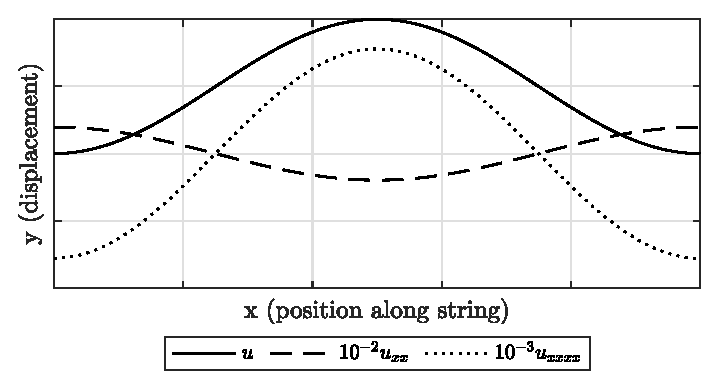
\includegraphics[width=\linewidth]{diffplot.eps}
  \label{fig:diffplot}
  \caption{Plot of a string $u = u(t, x)$ (solid line) and its derivative $u_{xx}$ (dashed line), which determines the force due to tension and $u_{xxxx}$ (dotted line), which determines the force due to stiffness.}
\end{figure}

The multiplicative term $T_0 + \frac{E A}{2L} \int u_x^2 dx$ of course involves the tension $T_0$ --- a higher tension will result in a stronger restoring force.
The integral part can be interpreted as the increase in tension that arises due the the increased length of the string at large displacements\cite[Chapter~5]{fletcher_physics_1998}.
This give rises to phenomena such as downwards pitch glides which you can experience by plucking e.g. a guitar string very hard.

The next term is the one involving $u_{xxxx}$, which is an expression of the force due to the stiffness of the string material.
A derivation of this can be found in \cite[Chapter~2]{fletcher_physics_1998}.
Looking at Figure \ref{fig:diffplot}. we see that $u_{xxxx}$ points in the same direction as $u$, notice then the minus in front of the term in equation (\ref{eq:stiffNonlinearString}), which means the stiffness will somewhat counteract the displacement of the string (but not in the same way as the tension).
Stiffness causes dispersion which gives rise to inharmonic overtones, which can be observed in e.g. a piano string or metal rods.

The term $-2 \sigma_0 u_t$ causes dampening of the system that, greatly simplified, occurs due to viscous air flow, internal friction, and radiated energy\cite[Chapter~2]{fletcher_physics_1998}. 
$u_t$ is the velocity of $u$, and is a vector pointing in the direction $u$ is currently $moving$, so adding a force opposite of this will intuitively cause dampening.
Higher velocities will cause a stronger dampening force which results in a exponential decrease in volume over time.

The term $2 \sigma_1 u_{txx}$ causes frequency dependent dampening of the string.
This addition does not really have any physical justification, but causes the correct perceptual phenomena of higher frequencies dying out more quickly\cite{bensa_simulation_2003}.
The part $u_{txx}$, the change in curvature over time, is less easy to understand intuitively and I have so far not found a good explanation of exactly why it works.

Proceeding with the discretization of Equation (\ref{eq:stiffNonlinearString}), we replace the derivative operators with suitable finite difference operators to get
\begin{align}
  \begin{split}
    \delta_{tt} u^n_l &= \frac{1}{M} \left(T_0 + \sum^{i-1}_{i=0} (\delta_{x+} u^n_i)^2 \right)\delta_{xx} u^n_l - \frac{E I}{M} \delta_{xxxx} u^n_l\\
    &- 2 \sigma_0 \delta_{t\cdot} u^n_l + 2 \sigma_1 \delta_{t-} \delta_{xx}u^n_l + \frac{1}{M} F.
  \end{split}
\end{align}

The new finite difference operators are defined as
% at(l+2) - 4 * at(l+1) + 6 * at(l) - 4 * at(l-1) + at(l-2)
\begin{align}
  \delta_{tt} &= \frac{1}{k^2}(u^{n-1}_l - 2 u^n_l + u^{n+1}_l) \\
  \delta_{xx} &= \frac{1}{h^2}(u^n_{l-1} - 2 u^n_l + u^n_{l+1}),
\end{align}
which approximate $u_{tt}$ and $u_{xx}$,
\begin{align}
  \delta_{xxxx} = \frac{1}{h^2}(u^n_{l-2} - 4 u^n_{l-1} + 6 u^n_l - 4 u^n_{l+1} + u^n_{l+2})
\end{align}
which approxmiates $u_{xxxx}$, and
\begin{align}
  \delta_{t\cdot} &= \frac{1}{2k} (u^{n+1}_l - u^{n-1}_l) \\
  \delta_{t-} &=\frac{1}{k} (u^{n}_l - u^{n-1}_l)
\end{align}
that are both approximations of $u_t$

To actually compute the solution of our string model we must derive an \textit{update rule} or \textit{recurrence equation}, which will allow us to compute the state at the next time step $u^{n+1}_l$ from the current and past states.

We do this by expanding all operators that contains $u^{n+1}_l$ and then proceed isolate $u^{n+1}_l$ to get
\begin{align}
  \label{eq:stringUpdate}
  u^{n+1}_l &= \frac{1}{1 + k\sigma_0} (F_t + F_s + F_d + F_e + 2u^n_l - u^{n-1}_l)
\end{align}
where
\begin{align}
  F_t &= \frac{k^2}{M} \left(T_0 + \sum^{L-1}_{i=0} h(\delta_{x+} u^n_i)^2 \right)\delta_{xx} \\
  F_s &= -\frac{k^2 E I}{M} \delta_{xxxx} u^n_l\\
  F_d &= k\sigma_0u^{n-1}_l + 2k\sigma_1 (\delta_{xx}u^n_l - \delta_{xx}u^{n-1}_l)\\
  F_e &= \frac{k^2}{M}F.
\end{align}
Notice we did not expand the spatial difference operators because the have no influence on the isolation of $u^{n+1}_l$, though could perhaps expand them and reduce the above equation to fewer operations, but I tend to prefer clarity over brevity.

Since our string should not be infinite it needs to end somewhere.
We will need to choose an integer $N$, which is the number of points on our string, each spaced by $h$.
Assuming that the length of our string is $1m$ we have $N = 1 / h$.

Special care needs to be taken at the boundaries --- the points $l=0$ and $l=N-1$.
There are multiple ways of doing this depending on what behavior we want.
We will be using a clamped boundary condition, which means that the points at each end must satisfy\cite[Chapter~7]{bilbao_numerical_2009}
\begin{equation}
  u = u_x = 0,
\end{equation}
which can be implemented by introducing some \textit{virtual points} at positions $-2, -1, N$ and $N+1$.

To ensure the condition $u = 0$ we choose
\begin{equation}
  u_{-1} = u_{N} = 0.
\end{equation}
For $u_x = 0$ we apply a finite difference operator at $l = -1$ to get
\begin{equation}
  \delta_{t\cdot} u^n_{-1} = \frac{1}{2h}(u^n_0 - u^n_{-2}) = 0
\end{equation}
which means that
\begin{equation}
  u^n_{-2} = u^n_0.
\end{equation}
The same can be done for $u^n_N$ which results in $u^n_{N+1} = u^n_{N-1}$.

% u_{tt} &= \frac{1}{M} \left(T_0 + \frac{E A}{2L} \int u_x^2 dx \right)u_{xx} - \frac{E I}{M} u_{xxxx}\\
%   &- 2 \sigma_0 u_t + 2 \sigma_1 u_{txx} + \frac{1}{M} F

\subsection{Spring}
\label{sec:spring}

The springs which connect the string to the drum membranes is modeled with
\begin{align}
  \begin{split}
  u_{xx} &= -\kappa^2 u_{xxxx} \\
  & - 2 \sigma_0 u_t + 2 \sigma_1 u_{txx} + \frac{1}{M} F.
  \end{split}
  \label{eq:spring}
\end{align}
In this model $\kappa$ is a constant usually determined by scale, Young's modulus and moment of inertia of the material, but in this case unitless and corresponds roughly to pitch or echoes per second\cite{bilbao_modular_2009}\cite{parker_modeling_2010}.
$M$ is the mass of the spring, which we can choose independently of $\kappa$.

The informed reader will notice that Equation (\ref{eq:spring}) is actually the equation for the dynamics of a linear stiff bar\cite{bilbao_modular_2009}\cite[7]{bilbao_numerical_2009}.
However, it was also used by Parker, Penttinen, and Bilbao to model wave propagation on a slinky --- a long, large diameter spring --- so it should be suitable for modeling the springs of the Yaybahar as well\cite{parker_modeling_2010}.

There is no need to go over the terms of Equation (\ref{eq:spring}), because we have already seen all the terms before in Equation (\ref{eq:stiffNonlinearString}) and explained them in section \ref{sec:string}.
We should note though that there is no force due to tension, because the only restoring force in the spring is the material stiffness.

We discretize Equation (\ref{eq:spring}) by applying the suitable difference operators to get
\begin{equation}
  \begin{split}
  \delta_{xx} u^n_l &= -\kappa^2 \delta_{xxxx} u^n_l\\
  &- 2 \sigma_0 \delta_{t\cdot} u^n_l + 2 \sigma_1 \delta_{t-} \delta_{xx}u^n_l + \frac{1}{M} F.
  \end{split}
\end{equation}
Then, expanding the operators and isolating $u^{n+1}_l$ we get
\begin{equation}
u^{n+1}_l = \frac{1}{1 + k\sigma_0} (F_s + F_d + F_e + 2u^n_l - u^{n-1}_l)
\end{equation}
where
\begin{align}
  F_s &= -k^2 \kappa^2 \delta_{xxxx} u^n_l\\
  F_d &= k\sigma_0u^{n-1}_l + 2k\sigma_1 (\delta_{xx}u^n_l - \delta_{xx}u^{n-1}_l)\\
  F_e &= \frac{k^2}{M}F.
\end{align}

At each end a spring is attached either to the string or to a drum head.
We will model this by using free boundary conditions and the connections covered in section \ref{sec:connections}.
Free boundary conditions means that at either end of the spring we must satisfy
\begin{equation}
  \label{eq:freeBoundaryCondition}
  u_{xx} = u_{xxx} = 0.
\end{equation}

This is implemented by first discretizing Equation (\ref{eq:freeBoundaryCondition}) using finite difference operators to get
\begin{equation}
  \label{eq:discretizedFreeBoundaryCondition}
  \delta_{xx} u^n_l = \delta_{x-}\delta_{xx} u^n_l = 0.
\end{equation}

If we expand Equation (\ref{eq:discretizedFreeBoundaryCondition}) for $l = 0$ we get
\begin{align}
  \frac{1}{h^2} (u^n_{-1} - 2 u^{n}_0 + u^{1}) &= 0 \label{eq:freeBoundaryDxx}\\
  \frac{1}{h^3} (-u^n_{-2} + 3u^n_{l-1} - 3u^n_0 - u^n_{1}) &= 0 \label{eq:freeBoundaryDxxxx}.
\end{align}
we then take Equation (\ref{eq:freeBoundaryDxx}) and solve for the first virtual point $u^n_{-1}$ to get
\begin{equation}
  u^n_{-1} = 2 u^n_0 - u^n_1.
\end{equation}
This can then be plugged into Equation (\ref{eq:freeBoundaryDxxxx}) so we can solve for $u^n_{l-2}$ which yields
\begin{equation}
  u^n_{-2} = 3 u^n_0 - 2u^n_1.
\end{equation}

We can do the same exercise for the right side to get
\begin{align}
  u^n_{N} &= 2 u^n_{N-1} - u^n_{N-2}\\
  u^n_{N+1} &= 3 u^n_{N-1} - 2 u^n_{N-2},
\end{align}
where $N$ is the number of points on our spring.

\subsection{Membrane}
\label{sec:membrane}
The drum heads of the Yaybahar can be modeled as two membranes under tension.
The equation for this is
\begin{align}
  \label{eq:nonlinearMembrane}
  \begin{split}
  u_{tt} &= \frac{1}{M} \left(T_0 + \frac{6D}{A H^2} \iint_A \nabla u^2 dA \right)\Delta u \\
  &- 2 \sigma_0 u_t + 2 \sigma_1 \Delta u_t + \frac{1}{M} F.
  \end{split}
\end{align}
where we have the displacement $u = u(x, y, t)$; $H$ is the thickness of the material, and $A$ is the surface area.
The parameter $D$ is defined by
\begin{align}
  D = \frac{E H^3}{12 (1 - \nu^2)},
\end{align}
which is called the \textit{flextural regidity} of the membrane. Again, $E$ is the Young's modulus of the material and $\nu$ is Poisson's ratio, which determines how the material deforms under strain.
The model in Equation (\ref{eq:nonlinearMembrane}) is based on the 2D wave equation and nonlinear plate vibration covered in \cite[Chapters~11, 12, and 13]{bilbao_numerical_2009}.

You might have noticed that Equation (\ref{eq:nonlinearMembrane}) is very similar to (\ref{eq:stiffNonlinearString}) except now in two dimensions.
In fact, the forces in both equation arise due to the same phenomena.
Notice also that our membrane has no stiffness.
This is because we assume that it is made from some non-stiff material such as hide or plastic.

Because we are now working with a 2D system we need to be aware of spatial derivatives in two directions.
This is why we have the gradient, defined as
\begin{equation}
  \nabla u = u_x + u_y,
\end{equation}
and the laplacian, defined as
\begin{equation}
  \Delta u = u_{xx} + u_{yy}.
\end{equation}

At this point we are assuming cartesian coordinates, however, since the drums of the Yaybahar are round, we might also want to make the domain of our model round.
This can be done by expressing positions radial coordinates, radius $r$ and angle $\theta$, instead of $x$ and $y$.
By expressing our cartesian coordinates using our radial ones
\begin{align}
  x &= r \cos \theta\\
  y &= r \sin \theta,
\end{align}
we can transform our derivatives into radial coordinates as well.
E.g. we can show the laplacian in radial coordinates is
\begin{equation}
  \Delta u = u_{rr} + \frac{1}{r} u_{rr} + \frac{1}{r^2} u_{\theta \theta}.
\end{equation}

However, we are not going to do this because finite difference schemes in radial coordinates, especially the efficient, \textit{implicit} ones, have a tendency to misbehave \cite[Chapter~12]{bilbao_numerical_2009}.
The main problem for our case is that the sound will be severely band limited, which will kill the tone of our assembled Yaybahar model, so we will stay in cartesian coordinates.

Equation (\ref{eq:nonlinearMembrane}) can be discretized like this
\begin{align}
  \label{eq:nonlinearMembraneFds}
  \begin{split}
  \delta_tt u^n_{l, m} &= \frac{1}{M} \left(T_0 + \frac{6D}{A H^2} \sum_{x, y} h_x h_y (\delta_\nabla u^n_{l, m})^2 \right)\delta_\Delta u^n_{l, m} \\
  &- 2 \sigma_0 \delta_{t\cdot} u^n_{l, m} + 2 \sigma_1 \delta_\Delta \delta_{t-} u^n_{l, m} + \frac{1}{M} F.
  \end{split}
\end{align}
using the definitions
\begin{align}
  \delta_\nabla u^n_{l, m} &= \delta_{xx} u^n_{l, m} + \delta_{yy} u^n_{l, m}\\
  \delta_\Delta u^n_{l, m} &= \delta_{x+} u^n_{l, m} + \delta_{y+} u^n_{l, m}
\end{align}

Expanding the operators in Equation (\ref{eq:nonlinearMembraneFds}) and solving for $u^{n+1}_{l, m}$ we get 
\begin{align}
  u^{n+1}_{l, m} = \frac{1}{1 + k\sigma_0} (F_s + F_d + F_e + 2 u^n_{l, m} - u^{n-1}_{l, m})
\end{align}
where
\begin{align}
  F_s &= k^2 \frac{1}{M} \left(T_0 + \frac{6D}{A H^2} \sum_{x, y} h_x h_y(\delta_\nabla u^n_{l, m})^2 \right)\delta_\Delta u^n_{l, m} \\
  F_d &= k \sigma_0 u^{n-1}_{l, m} + 2 k \sigma_1 (\delta_\Delta u^{n+1}_{l, m} - \delta_\Delta u^{n-1}_{l, m}) \\
  F_e &= \frac{k^2}{M} F
\end{align}

As for boundary conditions, we now have the four edges around our membrane we need to take care of\footnote{Even though we are using cartesian coordinates the shape of our membrane does not need to be rectangular, but for now that is what we choose it to be.}.
Like with the string we will use a clamped boundary conditions which means that we define virtual points
\begin{equation}
  u^{n+1}_{l, m} = 0,
\end{equation}
along all edges, that is, when $l = -1$, $l = N_x$, $m = -1$, or $m = N_y$, where $N_x$ and $N_y$ are the number of points in each direction.

\subsection{Bow}
\label{sec:bow}

A bow, like the one used to play the Yaybahar, works by the friction between the bow hairs and the resonater being played, in this case a string.
At first the bow will pull the string along, but at some point the restoring force in the string becomes too large and the string shoots back only to be caught by the bow again \cite[Chapter~2]{fletcher_physics_1998}.
The frictional force between the bow and the string is determined in part by the relative velocity between them.

We model this by using the model from \cite[Chapter~4]{bilbao_numerical_2009}, where we apply a force $F$ to our system in Equation (\ref{eq:stiffNonlinearString}) that is determined by
\begin{equation}
  \label{eq:bowForce}
  F = - F_b \phi(v_{rel}),
\end{equation}
where
\begin{equation}
  v_{rel} = u_t - v_b.
\end{equation}
Here $F_b$ is the force in Newtons at which the bow is pressed down onto the string, $v_{rel}$ is the relative velocity of the bow to the string at the bowing point with $v_b$ being the bow velocity in $m/s$.

There are many ways of defining $\phi$, but we will be using the definition
\begin{equation}
  \label{eq:phi}
  \phi(v_{rel}) = \sqrt{2a} v_{rel} e^{-a v_{rel}^2 + 1/2},
\end{equation}
where $a$ is a dimensionless constant that determines the shape of the function.
A plot of $\phi(v_{rel})$ can be seen in Figure \ref{fig:bowplot}.

\begin{figure}[h]
  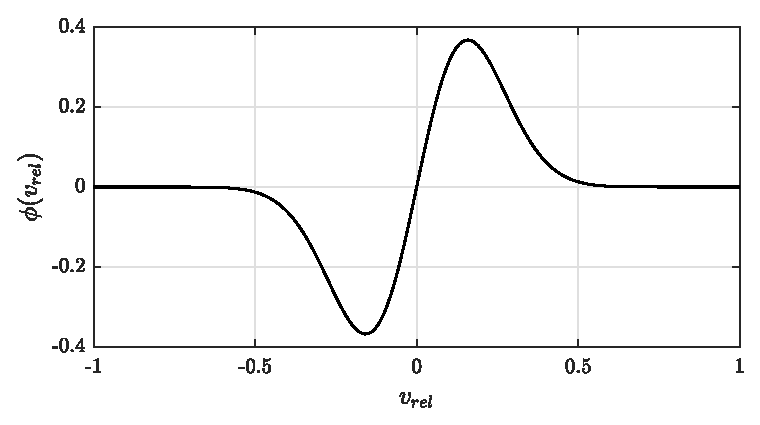
\includegraphics[width=\linewidth]{bowplot.eps}
  \label{fig:bowplot}
  \caption{A plot of $\phi(v_{rel})$ of Equation (\ref{eq:phi}) with $a = 20$}
\end{figure}

To implement our bow model we must discretize Equation (\ref{eq:bowForce}), which means discretizing $v_{rel}$.
We will do this using the scheme
\begin{equation}
  \label{eq:vrelScheme}
  v_{rel} = \delta_{t\cdot} u^n_{l_b} - v_b,
\end{equation}
where $l_b$ is the index of our bowing point.

If we expand Equation (\ref{eq:vrelScheme}) we get
\begin{equation}
  \label{eq:vrelSchemeExpanded}
  v_{rel} = \frac{1}{2k}\left(u^{n+1}_{l_b} - u^{n-1}_{l_b}\right) - v_b.
\end{equation}
Notice that $v_{rel}$ depends on $u^{n+1}_{l_b}$, but to compute $u^{n+1}_{l_b}$ using Equation (\ref{eq:stiffNonlinearString}) combined with Equation (\ref{eq:vrelScheme}) we need $v_{rel}$.
This cyclic dependency results in what we call an \textit{explicit} scheme which we can only solve using \textit{iterative methods}.

One such method is the Newton-Raphson method which says that if we have a function $f(x) = 0$, then we can get continuously better results for $x$ by iteratively doing
\begin{equation}
  x \leftarrow x - \frac{f(x)}{f_x(x)},
\end{equation}
where we keep going until the change in $x$ is sufficiently small.

We apply this by first putting Equation (\ref{eq:vrelSchemeExpanded}) into the correct from
\begin{equation}
  f(v_{rel}) = \frac{1}{2k} \left(u^{n+1}_{l_b} - u^{n-1}_{l_b} \right) - v_b - v_{rel} = 0.
\end{equation}
Then we substitute $u^{n+1}_{l_b}$ using Equation (\ref{eq:stringUpdate}) and take the derivative of it all with respect to $v_{rel}$ to get
\begin{equation}
  f_{v_{rel}}(v_{rel}) = - \frac{1}{2k} k^2 F_b \phi_{v_{rel}}(v_{rel}) - 1.
\end{equation}
where
% sqrt2a * (exp(-a * pow2(eta) + 0.5) - 2 * a * pow2(eta) * exp(-a * pow2(eta) + 0.5))
\begin{equation}
  \phi_{v_{rel}}(v_{rel}) = \sqrt{2 a} \left(e^{-a v_{rel}^2 + 1/2} - 2 a v_{rel}^2 e^{-a v_{rel}^2 + 1/2} \right).
\end{equation}
And thus, we have everything we need to iteratively compute $v_{rel}$.

Note that iterative methods can have a large impact on the efficiency of our synthesis algorithm --- not great for the prospect of having it run in real-time.
In the current case, however, it is not too bad since we only need to run the solver for the bowing point $l_b$ and not for every point on our string.

\subsection{Connections}
\label{sec:connections}

To connect the elements of our Yaybahar we will use a simple spring-like connection.
Say that e.g. $u^n_{l_{uc}}$ is the connecting point on our string and $w^n_{l_{wc}}$ is the connecting point on one of the springs.
The force caused by the connection between them is defined by
\begin{equation}
  F_c = k \left(u^n_{l_{uc}} - w^n_{l_{wc}}\right),
\end{equation}
where $k$ is a positive constant determining the strength of the connection.

This connection scheme is basically just Hooke's law, but similar the e.g. the one found in \cite{bilbao_modular_2009}, where they also include non-linear terms.

After computing the connection force $F_c$ we simply apply it to our string and spring, but in opposite directions, so the string gets $F_c$ and the spring gets $-F_c$ added to their respective $F$ (external forces) in Equations (\ref{eq:stiffNonlinearString}) and (\ref{eq:spring}).

\section{Implementation}
\label{sec:implementation}

Everything covered in section \ref{sec:elements}. is implement in C++ and the code is available on GitHub\footnote{\url{https://github.com/pellejuul/yaybahar}, latest commit at time of writing: 039bf85}.
This section covers how the code is structured and which optimization were applied to make it run in real-time.

\subsection{Code Structure}

The code is structured in three layers of abstraction: domains, models, and application code.

Domains implement the low level details that are common for multiple models.
This encompasses arrays for holding models states, computation of boundary conditions, and routines for the various finite difference operators.
The following domain classes are implemented
\begin{description}
  \item[Domain1d] a 1D domain used for the string and spring models.
  \item[Domain2d] a cartesian 2D domain used for the drum membrane models. 
  \item[Domain2dRadial] a radial 2D domain used in an earlier round membrane model.
\end{description}

The model layer uses the domain layer to implement the models of section \ref{sec:elements}.
Using the domain classes allows the developer to focus on the high level aspects of the model without getting bogged down by e.g. the implementation of the finite difference operators.
The model classes implemented are
\begin{description}
  \item[BowedString] the string model from section \ref{sec:string}. combined with the bow model from section \ref{sec:bow}. using Domain1d.
  \item[Connection] the connection model from section \ref{sec:connections}.
  \item[RectMembrane] the membrane model from section \ref{sec:membrane}. using Domain2d.
  \item[Spring] the spring model of section\ref{sec:spring}.
\end{description}

The application code ties all the model classes together using the connection class, provides real-time audio output, and a GUI for controlling the relevant parameters of each model.

\subsection{Optimizations}
\label{sec:optimizations}

To make the full Yaybahar run in real-time the code needed to be optimized.
Three categories of optimizations were applied:
\begin{enumerate}
  \item Only compute what is needed.
  \item Pre-compute as much as possible.
  \item Avoid branches in critical parts of the code.
  \item Avoid memory allocation and copying.
  \item Compile with optimizations enabled (clang flag -O3).
\end{enumerate}

An example of optimization 1. can be found in the BowedString class, where we only need to iteratively compute $v_{rel}$ once.
We also avoid calling the routine for $\phi(v_{rel})$ unless necessary.

For optimization 2. we want to focus on constant terms that contain divisions or non-arithmetic functions, such as exponentials and square roots, since these take many clock cycles to compute.
Obvious targets for this is the term $1 / (1 + k\sigma_0)$ which appears multiple places, or $\sqrt{2a}$ in the bow model.

The reason for optimization 3. is that branches can severely slow down our code.
Branches, such as if-statements, can cause our processor, which is doing branch prediction, to have to clear its pipeline, resulting in a delay of multiple clock cycles.
One example of this with boundary conditions: a naive implementation could use if-statements to check if we are at the boundary, resulting in multiple branches for each point in our domain.
Instead, we can use a bit more memory and pre-compute the virtual points along the boundary, thus avoiding branches.

Heap memory allocation and deallocation, e.g. malloc, new, or free, can take an indeterminate amount of time and should be avoided in critical code (optimization 4.).
A naive implementation of e.g. the string model would have three state arrays \lstinline{u}, \lstinline{un}, and \lstinline{up} representing the current, next, and previous states. After computing \lstinline{up} using the update rule it would copy the values of the arrays like so:
\begin{lstlisting}[language=C++]
for (int i = 0; i < N; i++)
{
  up[i] = u[i];
  u[i] = un[i];
}
\end{lstlisting}
The actual implementation uses C++ references in a loop so memory copy is avoided.
The three arrays (actually domain instances) \lstinline{u}, \lstinline{un}, and \lstinline{up} are now references instead, so we can simply do
\begin{lstlisting}[language=C++]
  Domain1d &uswap = up;
  up = u;
  u = un;
  un = uswap;
\end{lstlisting}
which is nearly instant.

Lastly (optimization 5) one of course have to enable compiler optimizations, which usually cases a speedup much higher than what a programmer could expect to achieve by hand.

There are of course more optimizations that one could do.
For example on can use C++ templates and compile time execution to help the compiler optimize the code even more.
One could also use vectorization which can greatly speed up the computation, but doing so will usually also decrease code clarity and portability. 

\section{Conclusion}
\label{sec:conclusion}

In this paper we have covered how to build a physical modeling sound synthesis algorithm for a specific instrument: the Yaybahar.

After a brief review of finite difference schemes we went through each element of the instrument, a bowed string, springs, and drum membranes, discussed their physics, and showed to how implement numerical simulations of them using finite difference schemes.

The implementations was implemented as a C++ application structured in three layers: domains, that took care of low level details, models, which implemented the models of the elements, and application, which tied everything together in an interactive real-time fashion.

For the purpose of real-time synthesis we covered some of optimizations, most of them C++ specific, that was applied to the code.

It is the hope of the author that this paper may inspire other people to pursue physical modeling of musical instruments using finite difference schemes in a way that will enrich the academic community and the world of sound and music in general.

%%%%%%%%%%%%%%%%%%%%%%%%%%%%%%%%%%%%%%%%%%%%%%%%%%%%%%%%%%%%%%%%%%%%%%%%%%%%%
%bibliography here
\bibliography{rsmc}

\end{document}
